\setcounter{chapter}{5}


\chapter{Evaluating a Semantic-based Automated Approach to Task-Relevant Text Identification}
\label{ch:assisting}


In the last chapter, we showed that semantic-based approaches can help identify text in artifacts relevant to a task. 
In this chapter, we consider whether one of these approaches---\textit{BERT with no filters}---can assist a software developer while they \textit{work} on a task.


To perform this evaluation, we embed the BERT with no filters approach into a web browser plug-in that  highlights 
text relevant to a particular software task in web pages inspected by a developer.
We investigate whether this tool, which we call \acs{tool}, aids developers through a controlled experiment,
thus addressing whether developers can effectively complete a software task 
when provided with task-relevant text  extracted from natural language artifacts. 
We report how  24 participants completed three Python programming tasks 
with and without \acs{tool}.
Our results show that participants considered the majority of the text  identified automatically in the artifacts 
they perused useful and that 
the tool assisted them in producing a more correct solution for one of the experimental tasks.



We start by outlining the evaluation approach  (Section~\ref{cp6:method}). We then
detail experimental procedures  (Section~\ref{cp6:experiment}) before reporting
results from the experiment 
(Section~\ref{cp6:results}).
Section~\ref{cp6:summary} concludes the chapter.






\section{Motivation}
\label{cp6:method}



Our goal is to examine how \acs{tool}---a tool that 
 identifies
task-relevant text in pertinent
documents automatically---can affect a developer's work.
Building on work presented earlier in this
thesis, the tool  uses the BERT with no filters semantic-based technique.
By identifying information that is useful to the developer's task,
a developer's burden to find task-relevant information~\cite{Robillard2015}
can be lowered,
allowing them to focus their time on other activities such as judging how the information found applies to their task.


To be helpful, \acs{tool} must direct a developer's attention to text that assists them in completing a task.
If the tool is successful in identifying text useful to the task, we hypothesize that
the developer will produce a correct solution more often than if they had not used the tool.


Even if a developer is more successful
with the tool than without, there is a chance that the text shown by \acs{tool} is not \textit{useful}---either because it is not relevant for the task at hand or because it is unsurprising, i.e.,
a developer finds the text identified by the tool as ``common-knowledge''~\cite{cwalina2008, Robillard2015}. Our experimental design incorporates the gathering of qualitative data to assess the usefulness of the text identified.

 







\section{Experiment}
\label{cp6:experiment}



\gcm{The figure would be better as a summary rather than introducing the chapter.}

\gcm{Are there research questions?}

Figure~\ref{fig:tool-experiment-procedures} presents an experiment designed to evaluate how a semantic-based tool might assists a software developer perform a task.
In this experiment, 24 participants with software development background each attempted a
\textit{control} and \textit{tool-assisted} task randomly drawn from a list of well-known Python programming tasks.
Participants are asked to write a solution for both of their assigned tasks
and we use the control task to collect what text a participant deems relevant to the task at hand.
In the tool-assisted task, we gather input on the usefulness of the text automatically identified and shown by our tool. 
This design---detailed in the following subsections---allow us to:




\begin{itemize}
    \item assess the correctness of the tasks performed \textit{with} or \textit{without} tool support;
    \item compare  the text that participants manually indicated as relevant in a certain artifact to the text automatically identified
    and shown by our tool for that same artifact, and;
    \item discuss the usefulness of the text automatically identified  according to the feedback provided by the participants.
\end{itemize}
 
\gcm{I suggest de-emphasizing the comparison of the text identification.}




\begin{figure}
\centering
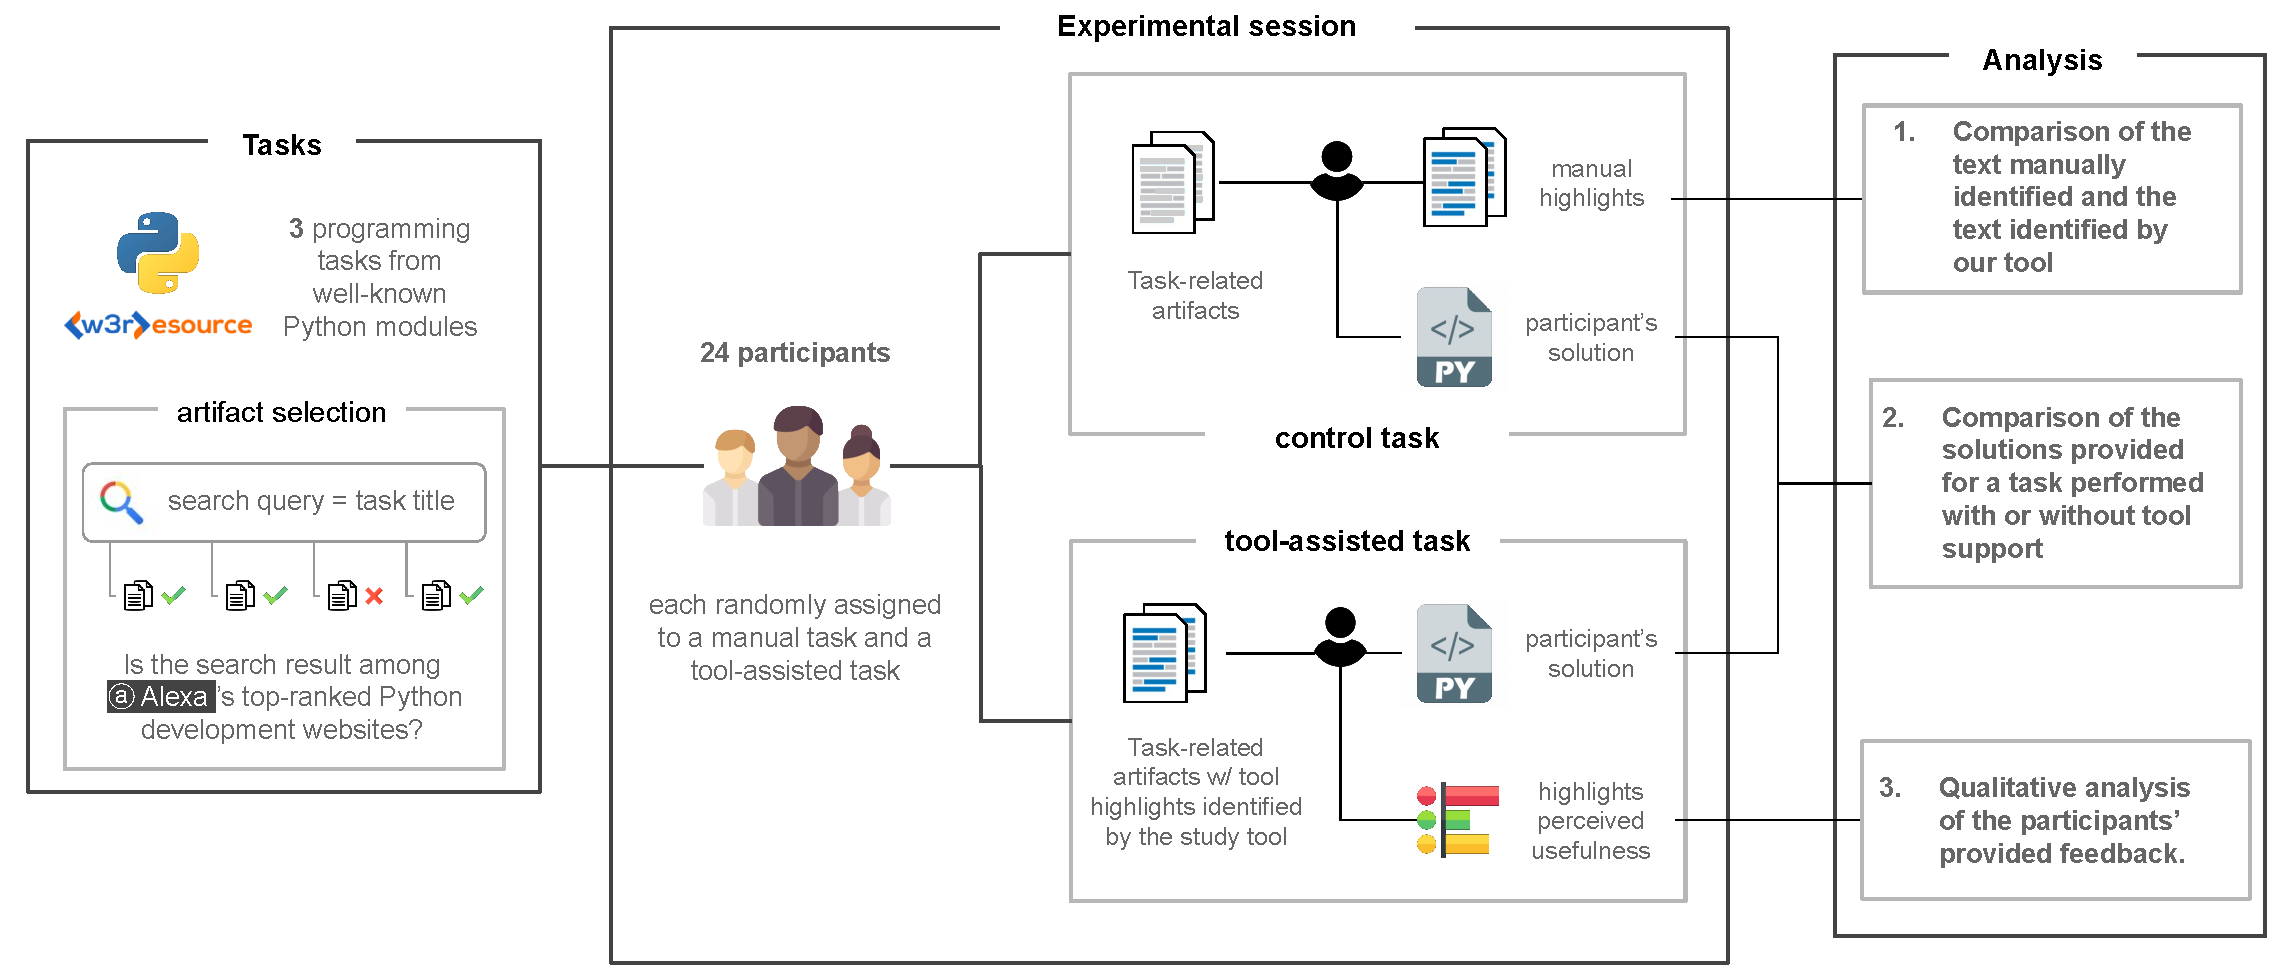
\includegraphics[width=1.0\textwidth]{cp6/tool-experiment-pipeline.pdf}
\caption{Summary of experimental procedures}
\label{fig:tool-experiment-procedures}
\end{figure}






\subsection{Study tool}



To automatically identify text that is potentially relevant to a developer's task, we have implemented 
a web browser plug-in that embeds one of our semantic-based approaches that we have previously explored, i.e., \textit{BERT with no filters}.

\gcm{Why not just name the approach in the chapter?} \art{TODO}


Our plug-in takes a developer's task and a software artifact as inputs and then applies its underlying semantic-based technique  to identify sentences that likely contain information useful to the input task.
The tool then highlights the text identified so that a developer can quickly located it amidst the rest of the content of an artifact  under inspection. 


We configure \textit{BERT with no filters} to identify no more than 10\% of the sentences of an input artifact as relevant.
This number was determined based on the average number of sentences indicated as relevant by human annotators in the artifacts of the \acs{DS-android} corpus.


\subsection{Tasks}
\label{cp6:tasks}

% \gcm{Was one of the three tasks used for a training task? I'm confused
% how many responses there were for each task.}

We opted for an experiment with tasks that could be completed by participants on their own time and computer.
This decision was motived by the COVID-19 pandemic and challenges related to recruiting participants and conducting an in-person experiment~\cite{russo2021a, russo2021b}. 
Since participants would follow instructions on their own, we decided to use tasks that are easy to understand and perform in a single experimental session, but that still required a participant  
to seek information in artifacts associated with each task.


Table~\ref{tbl:python-tasks-modules} details the tasks that we have selected based on task selection procedures from related work that meet these criteria~\cite{thiselton2019}. 
These tasks were drawn from
Python w3resource\footnote{\url{https://www.w3resource.com/python-exercises/}} tasks
that require usage of at least one module external to the Python core library.
By using external modules, we aim to reduce the likelihood that a participant 
can provide a solution for a task without consulting any of the artifacts (Section~\ref{cp6:experiment-artifacts})
that detail each of the modules associated with each task. 


Figure~\ref{fig:nytimes-task-github} provides an excerpt of the information shown in a task\footnote{Full descriptions are available in the experiment's supplementary material~\red{\cite{a}}.}.
For each task, participants had the task description and examples of input and output scenarios at their disposal. A task contained a list of resources that participants could consult 
so that they could write their solution.
Each task also contained a link to an online coding environment (Section~\ref{cp6:coding-environment})
where a participant could write and test their solution. 









\subsection{Artifacts}
\label{cp6:experiment-artifacts}


% Note that our decision to control the artifacts shown per task relates to our need to study if there is overlap between the text that participants manually identify as relevant and the text that our semantic-based tool identifies for these same artifacts. 


Each task requires a set of artifacts that a participant could peruse for information that could assist them in writing their solution.
Ideally, participants could find these artifacts on their own. However, our need to compare solutions between participants who perform a task 
assisted by our tool and without it as well as our need to compare the text that participants deem relevant to the text
automatically identified by our tool means that all participants must have the exact same artifacts for a task.


Therefore,
we follow procedures similar to the ones we used to create the \acs{DS-android} dataset to produce the list of artifacts for each of the tasks in Table~\ref{tbl:python-tasks-modules}. 
That is, we use the Google search engine to obtain up to ten artifacts that likely contain 
information that could help a participant correctly complete that task. 
Three pilot runs ensured that the artifacts collected using such procedures had sufficient information to complete a task without 
the need of additional resources. Based on these pilots, we simplified the description of the \texttt{distances} tasks removing the need to sort the list suggested addresses, what also led to the removal of two artifacts associated with sorting. Table~\ref{tbl:python-task-distribution} details the kinds of artifacts per task.



\subsection{Coding environment}
\label{cp6:coding-environment}



To ensure that participants had the same conditions to perform each task
and also to minimize setup instructions, we used Google Colab\footnote{\url{https://colab.research.google.com/}} as our coding environment. \gcm{Say something here that Colab is an online coding
notebook or something.}


Colab provided participants with a code editor with amenities commonly found in modern IDEs, e.g., code completion and syntax highlighting. It also ensured that all the participants 
performed the tasks in the same Python version and it lifted 
burdens that could arise from installing dependencies associated with the external modules used in each of our tasks. 


Figure~\ref{fig:nytimes-task-colab} shows an example of the Colab coding environment. 
First it handled dependencies management and then, 
it presented a class containing a single method with a \texttt{TODO} block where 
participants should write their solution. 
The environment also provided a main function where participants could see the output
of their code. Alternatively, a participant could use test cases to test their solution
against the examples shown in each task description.




\begin{table}
\centering
\caption{Python tasks}
\begin{footnotesize}
\rowcolors{2}{}{lightgray}
\begin{tabular}{ll}
\hline
\textbf{Task} & \textbf{Description}                                                                                         \\
\hline
\hline
%
\parbox[l][1cm][c]{1cm}{Practice task}       &
\parbox[l][1cm][c]{11cm}{Given three dictionaries representing address books,
you must write an algorithm using the Python core \texttt{dict} module to merge them.}    \\
\hline
%
Distances     &
\parbox[l][1.3cm][c]{11cm}{Given a string representing a rendezvou point and a list of suggested picnic addresses
    you must write an algorithm using the \texttt{geopy} module to find the  picnic address closest to the rendezvou point.} \\
%
NYTimes       &
\parbox[l][1cm][c]{11cm}{Given a string representing the url for NY Times Today's,
    write an algorithm using the \texttt{BeautifulSoup} and \texttt{requests} modules to scrape all the headlines of that page.}
\\
%
Titanic       &
\parbox[l][1cm][c]{11cm}{Given a string representing a url for the titanic dataset,
    you must write an algorithm using the \texttt{pandas} and \texttt{seaborn} modules to create a barchart of the data.}    \\
    
\hline
\end{tabular}
\end{footnotesize}
% \smallskip
\label{tbl:python-tasks-modules}
\end{table}







\begin{table}
\centering
\caption{List of artifact types per task}
\begin{scriptsize}
\begin{threeparttable}
\rowcolors{2}{}{lightgray}
\begin{tabular}{llcllc}
\hline
\textbf{Task} & \textbf{Artifacts} & \textbf{Total} & \textbf{Task} & \textbf{Artifacts} & \textbf{Total}                                                                              \\
\hline
\hline
%
%
\parbox[l][0.5cm][c]{1cm}{Distances}    & API documents             & 2  & \parbox[l][0.5cm][c]{1cm}{NYTimes}      & API documents             & 3 \\
\parbox[l][0.5cm][c]{1cm}{}             & Stack Overflow posts      & 3 & \parbox[l][0.5cm][c]{1cm}{}             & Stack Overflow posts      & 3 \\
\parbox[l][0.5cm][c]{1cm}{}             & Miscellaneous web pages   & 3 & \parbox[l][0.5cm][c]{1cm}{}             & Miscellaneous web pages   & 4 \\
\hline

\parbox[l][0.5cm][c]{1cm}{Titanic}      & API documents             & 4 & \parbox[l][0.5cm][c]{1cm}{Practice\tnote{*}}      & API documents             & 1 \\
\parbox[l][0.5cm][c]{1cm}{}             & Stack Overflow posts      & 3 & \parbox[l][0.5cm][c]{1cm}{}             & Stack Overflow posts      & 2 \\
\parbox[l][0.5cm][c]{1cm}{}             & Miscellaneous web pages   & 3 \\
\hline


\end{tabular}
\begin{tablenotes}
    \item[*] smaller number of artifacts due to it being a practice task;
\end{tablenotes}
\end{threeparttable}
\end{scriptsize}
\label{tbl:python-task-distribution}
\end{table}










\clearpage

\begin{figure}
    \centering
    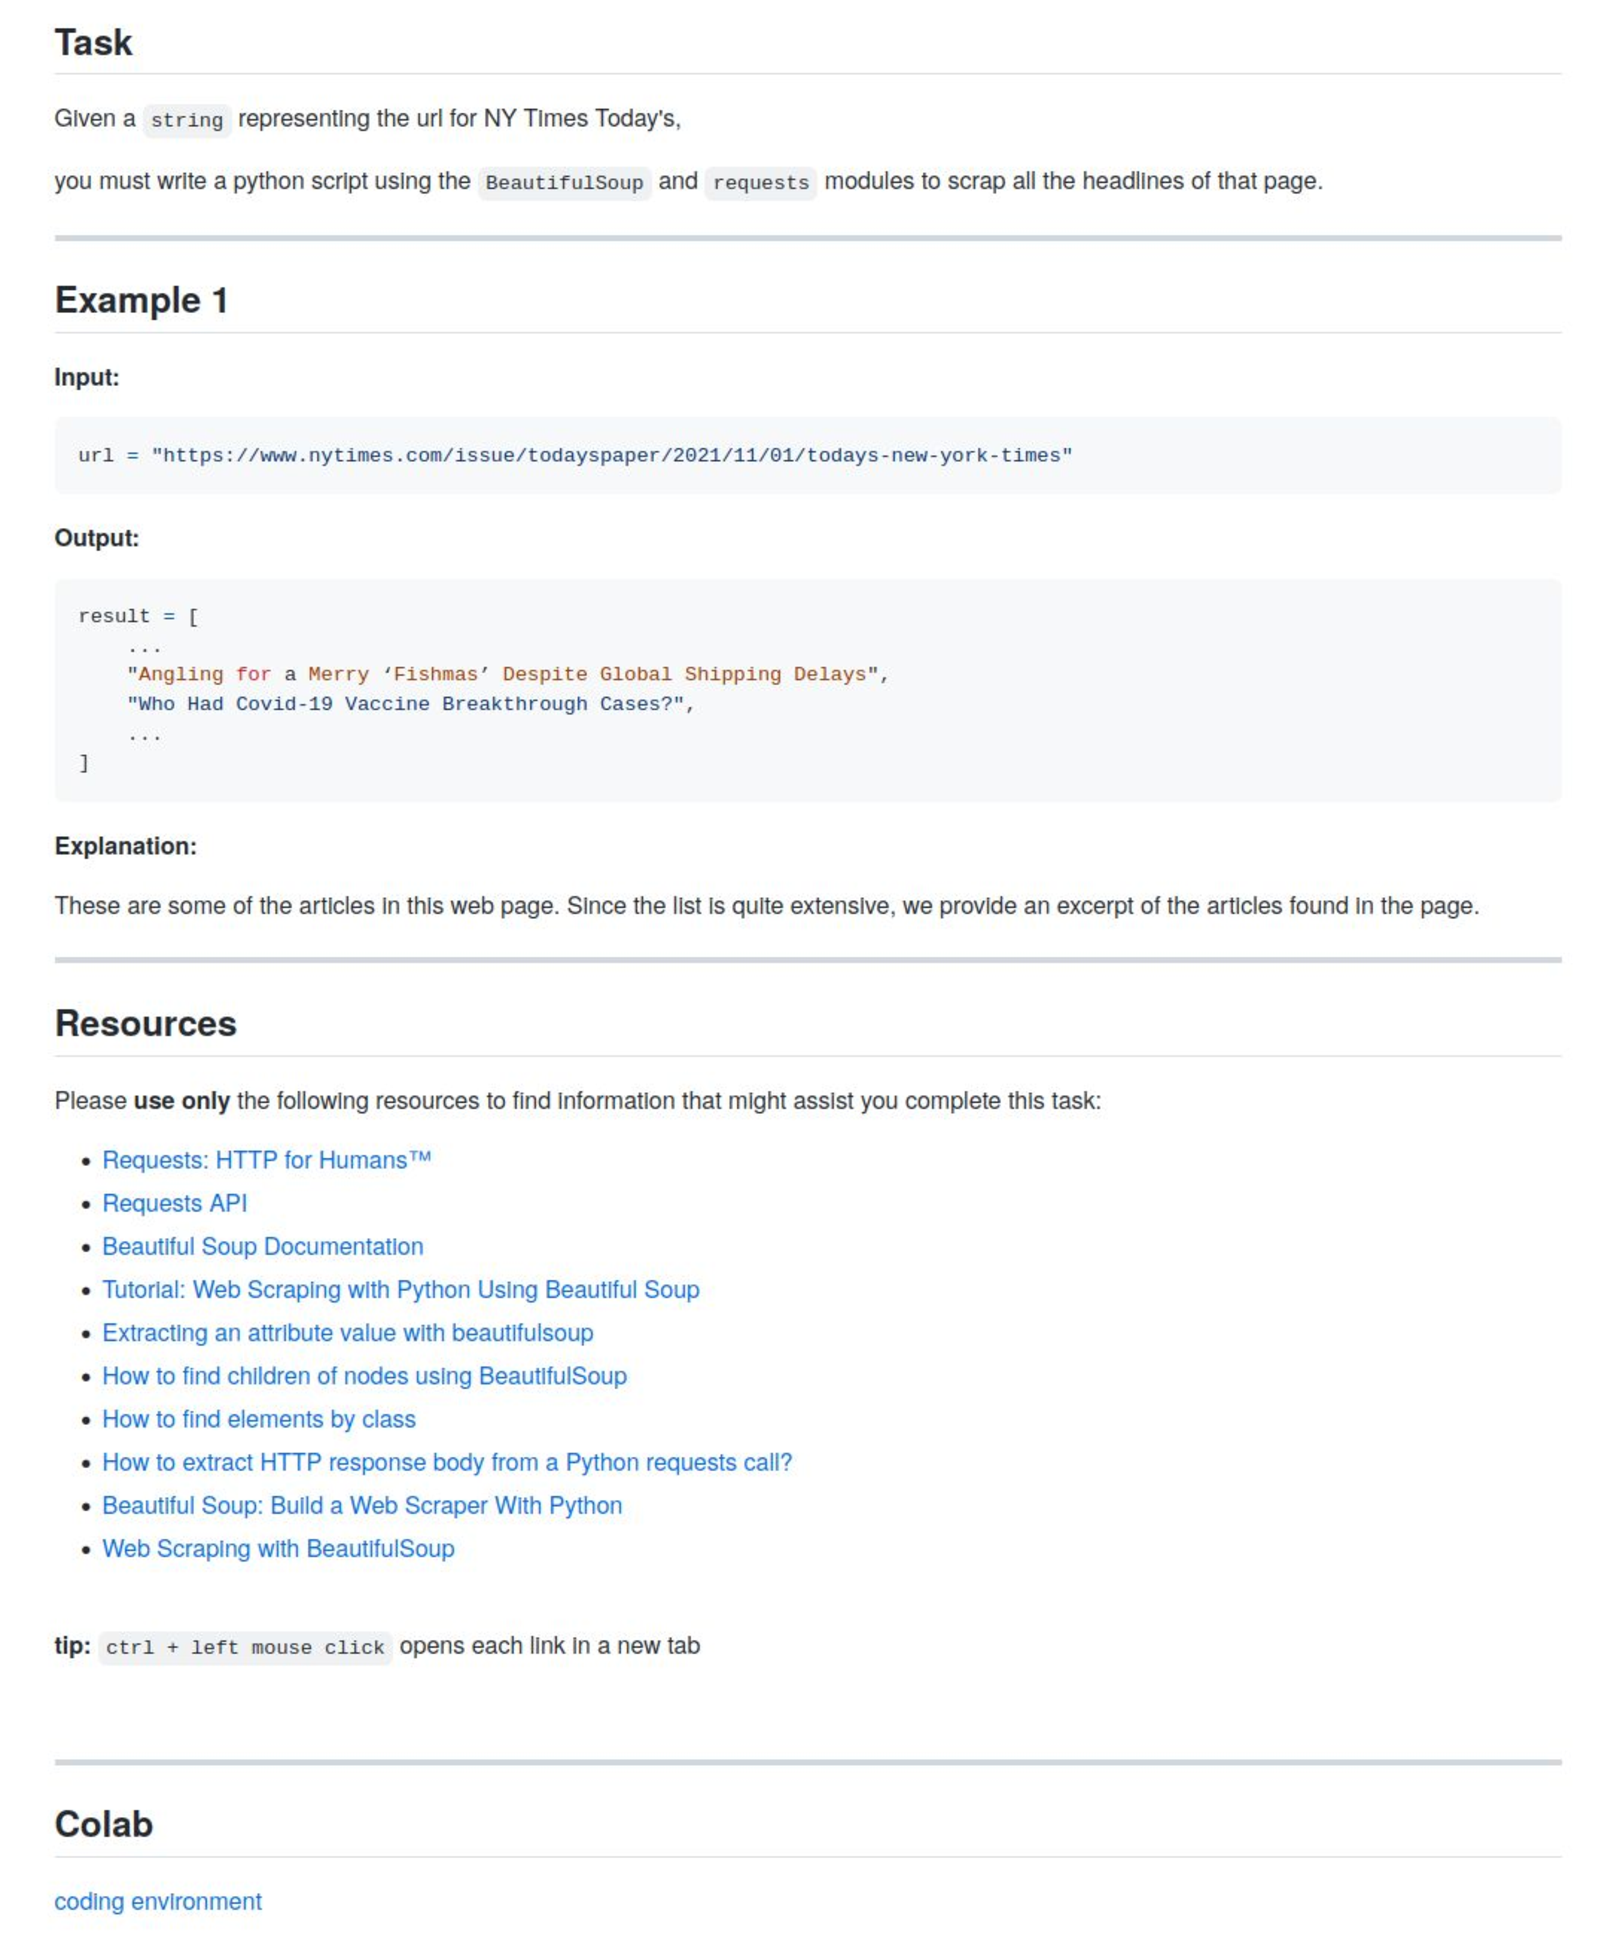
\includegraphics[width=1\textwidth]{cp6/task-github.pdf}
    \caption{Information shown in a task}
    \label{fig:nytimes-task-github}
\end{figure}



\clearpage

\begin{figure}
    \centering
    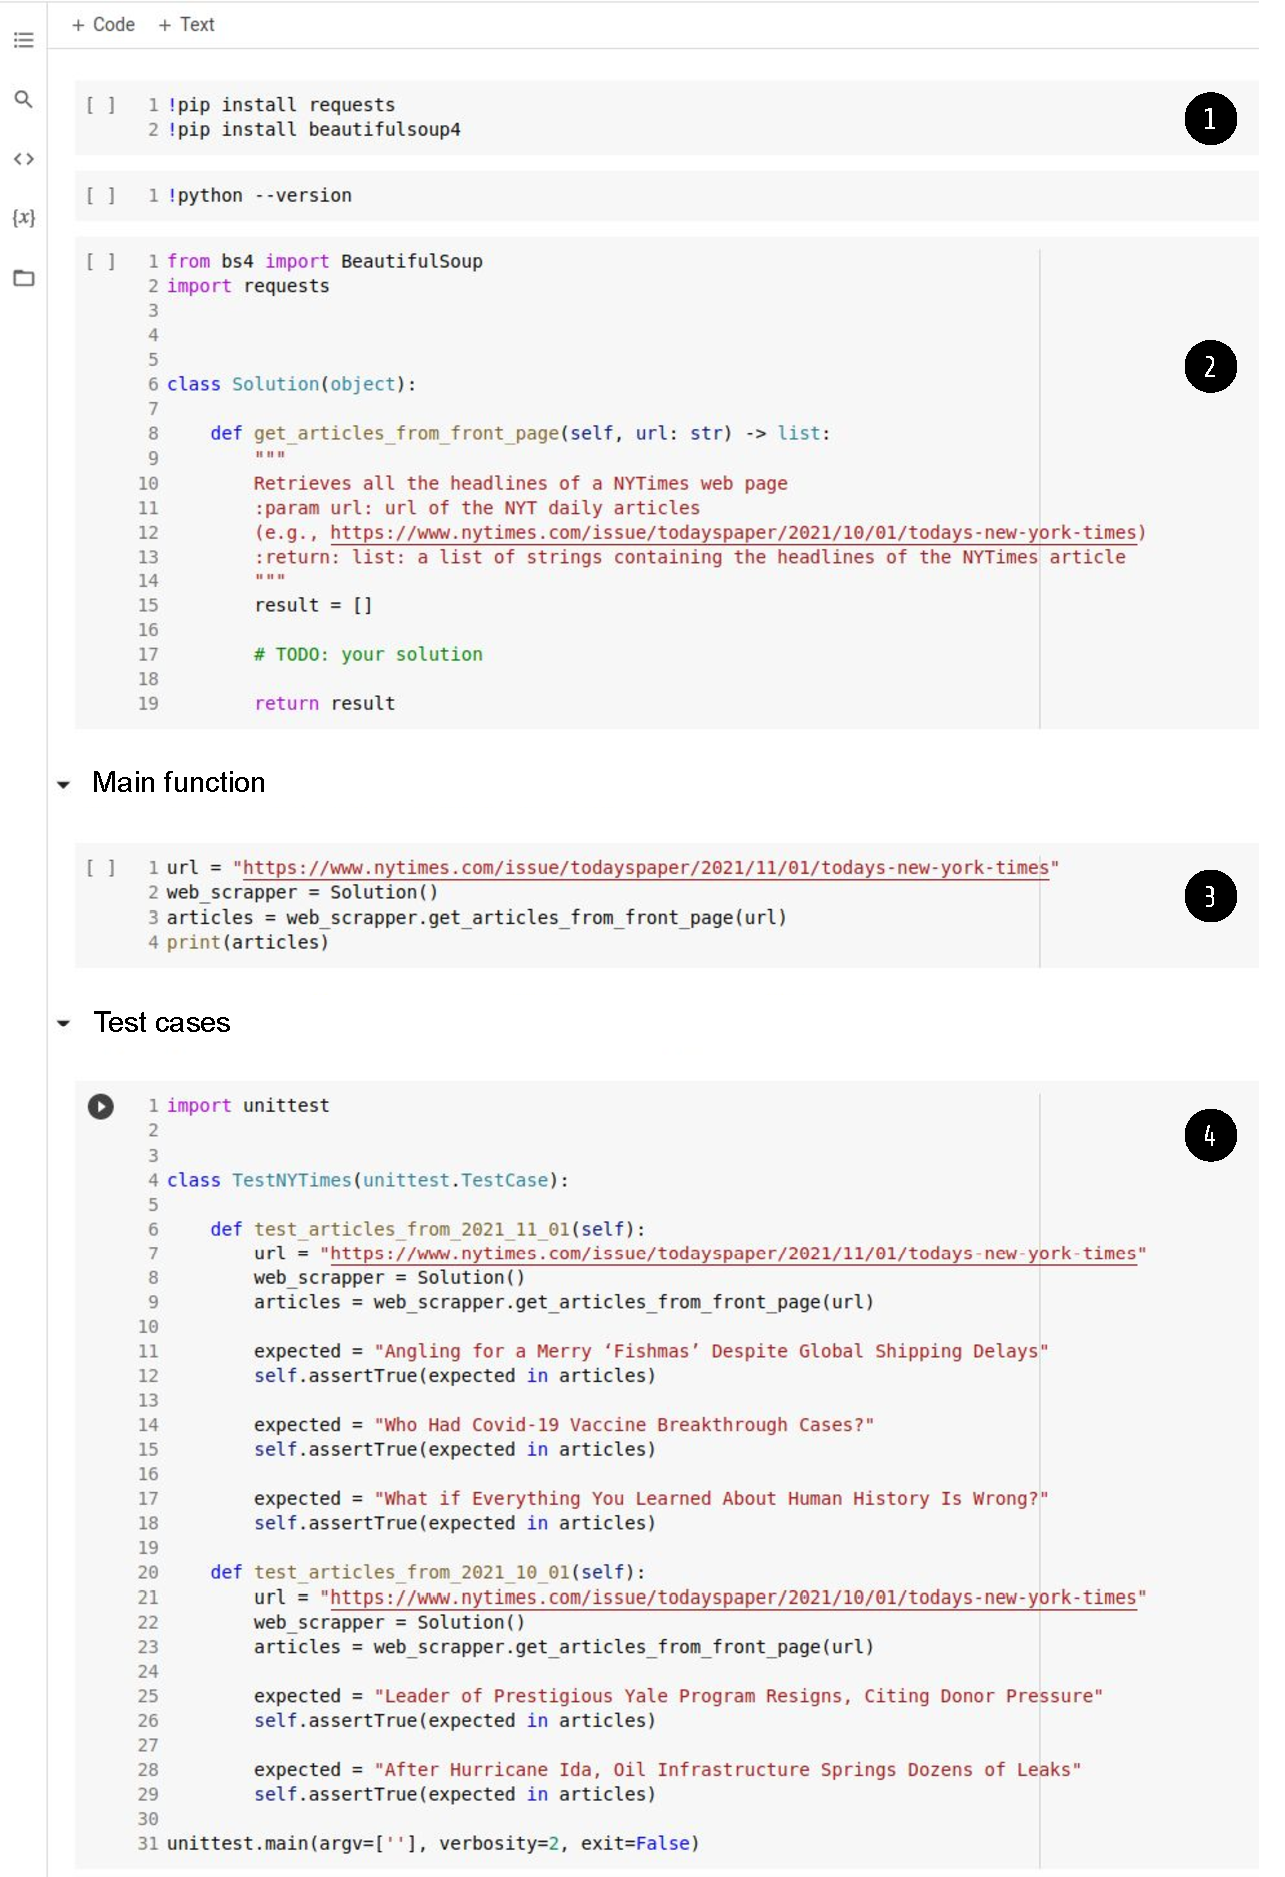
\includegraphics[width=\textwidth]{cp6/task-colab.pdf}
    \caption{Colab environment}
    \label{fig:nytimes-task-colab}
\end{figure}



\clearpage



\subsection{Participants}
\label{cp6:participants}


We advertised our study to professionals developers and to computer science students at  several universities. 
Our target population comprised professionals and third, fourth-year or graduate students.
We expected participants to have experience in Object-Oriented programming languages, and to consult API documentation when performing a programming task.
We gathered this background information as part of our demographics (Figure~\ref{fig:experiment-demographics})
and no participants were excluded
based on their background.

% \gcm{gender info?}



% (3 identified as female and 21 as male)


We obtained twenty four responses to our study advertisement (3 self-identified as female and 21 as male). 
At the time of the experiment, 10 participants were working as software
developers and 14 were students (11 graduate and 3 undergrad).
The majority of the students (71\%) also reported having some previous professional experience.


On average, participants self-reported 8 years of programming experience ({\small $\pm$} 3.8, ranging from 3 to 17 years).
The majority of the participants (54\%) had between 5 to 10 years of experience in Object-Oriented programming languages,
closely followed by participants  with  3 to 4 years of experience (29\%). 
Most of the participants also indicated that they did check API documents almost every time they performed a programming task. 


\begin{figure}
\begin{mdframed}[backgroundcolor=gray!15] 
\begin{scriptsize}

\noindent To witch gender do you identify? 

\medskip

\noindent If you are a student, in which year of the program are you at?  \smallskip

\quad $\square$~$1st$  
\quad $\square$~$2nd$  
\quad $\square$~$3rd$  
\quad $\square$~$4th$  
\quad $\square$~$5th+$ year 
\quad $\square$~\textit{graduate student} 

\medskip

\noindent For how many years have you been developing software?  

\medskip

\noindent For how many years have you been developing software \underline{professionaly}? 

\medskip

\noindent How many years of experience do you have in Object-Oriented programming languages?~\footnote{\scriptsize closed or open intervals notation} \smallskip

\quad $\square$~\textit{no experience} 
\quad $\square$ $(\infty, 1)$
\quad $\square$ $[1, 3)$
\quad $\square$ $[3, 5)$
\quad $\square$ $[5, 10)$
\quad $\square$ $[10, \infty)$

\medskip

\noindent With which frequency do you consult API documentation when performing a programming task?  \smallskip

\quad \textit{(never)} ~$1$ - $2$ - $3$ - $4$ - $5$ ~ ~\textit{(always)} 

\end{scriptsize}
\end{mdframed}
\caption{Background questions asked to a participant}
\label{fig:experiment-demographics}
\end{figure}

    



\gcm{earlier in the chapter you should probably cite the ethics certificate number the work was conducted under}
\art{should this go under the preface?}


\subsection{Procedures}
\label{cp6:procedures}




The entry point to our experiment was our advertisement email.
The email disclosed the purpose of the experiment, eligibility criteria, an estimate of the time it would take to complete it as well as a link 
to a web survey containing the experiment's consent form and tasks. 


Once a participant consented to participate, the survey gathered demographics and then, 
it gave participants further instructions 
about how to perform each task, requesting them to install the study tool, a web browser plug-in.
Setup was followed by a short practice task---separate from the experimental tasks---that allowed participants to familiarize themselves with the content of a task, the tool, and the coding environment that we used (Colab). 


Once a participant completed the practice task, the survey randomly assigned to them a \textit{control} task, which was followed by a randomly assigned \textit{tool-assisted} tasks---different from the control task.
For each task, including the practice tasks, the survey provided to the participants a link 
to the task description (Figure~\ref{fig:nytimes-task-github}) and asked them to submit a solution for the task, i.e., written Python code. Table~\ref{tbl:python-task-distribution} shows the participants who performed each task in the control and tool-assisted groups. While tasks were randomly assigned, we made sure that an even number of participants attempted a task with and without tool support.


Once a participant submitted their solutions, the survey
asked them about any additional feeback that they wished to share and 
offered them the opportunity to enter a raffle for one of two iPads 64 GB 
to compensate them for their time, what concluded the experiment.






\begin{table}[h!]
\centering
\caption{List of participants who performed each task}
\begin{footnotesize}
\rowcolors{2}{}{lightgray}
\begin{tabular}{lllc}
\hline
\textbf{Task} & \textbf{Configuration} & \textbf{Participants who attempted the task} & \textbf{\#}                                                                              \\
\hline
\hline
%
%
\parbox[l][0.5cm][c]{1cm}{Distances}
& \textit{control group}        & $P3, P4, P8, P12, P16, P17,  P21, P22$  & 8 \\
\parbox[l][0.5cm][c]{1cm}{}
& \textit{with tool support}    & $P1, P5, P9, P13, P15, P18, P20, P23, P24$ & 9 \\
\hline
%
%
\parbox[l][0.5cm][c]{1cm}{NYTimes}
& \textit{control group}     & $P1, P2, P6, P10, P11, P14, P15, P20$ & 8 \\
\parbox[l][0.5cm][c]{1cm}{}
& \textit{with tool support} & $P3, P7, P12, P16, P17, P19, P21,  P22$ & 8 \\
\hline
%
%
\parbox[l][0.5cm][c]{1cm}{Titanic}       
& \textit{control group}     & $P5, P7, P9, P13, P18, P19, P23, P24$ & 8 \\
\parbox[l][0.5cm][c]{1cm}{}
& \textit{with tool support} & $P2, P4, P6, P8, P10, P11,  P14$ & 7 \\
\hline
%
%
\end{tabular}
\end{footnotesize}
\smallskip
\label{tbl:python-task-distribution}
\end{table}

    







\subsubsection{Control Task}
\label{cp6:procedures-manual}

\gcm{Did they do this highlighting before the task or after? Confusing
to say 'study tool' - just say you asked them to highlight sentences.
'study tool' makes it sound like the tool being studied, i.e., the
one automaticalyl identifying text.}

In the \textit{control} task, we use the study tool to gather text that a participant deems useful for the task at hand. In this task, 
the survey asked participants to use the study tool to highlight sentences that they deemed useful and that provided information that assisted task completion---instructions similar to the ones used for the creation of the \acs{DS-android} corpus (Chapter~\ref{ch:android-corpus}).



Figure~\ref{fig:artifact-pre-highlight}
gives insight into how participants highlighted sentences using the study tool. 
Whenever a participant inspected one of the artifacts available for their task, 
they could click on the \texttt{highlight} button in the tool's context menu.  
This would then instrumented the HTML of the page identifying individual sentences. 
A participant could hover over identified sentences and select them as relevant by clicking on the hovered text.
Once a participant had finished selecting sentences, they could submit 
their data also through the tool's context menu.


% As an example, Figure~\ref{fig:artifact-pre-highlight} shows a sentence discussing the \texttt{find\_all} method, which 
% one of the participants in our experiment deemed 
% relevant to the \texttt{NYTimes} task.
% Based on the pilots, we observed that the most natural flow adopted by participants was to highlight text on-the-fly. That is, they indicated what text 
% was relevant for the task at hand while they consulted each artifact and wrote their solution. 



\begin{figure}
    \centering
    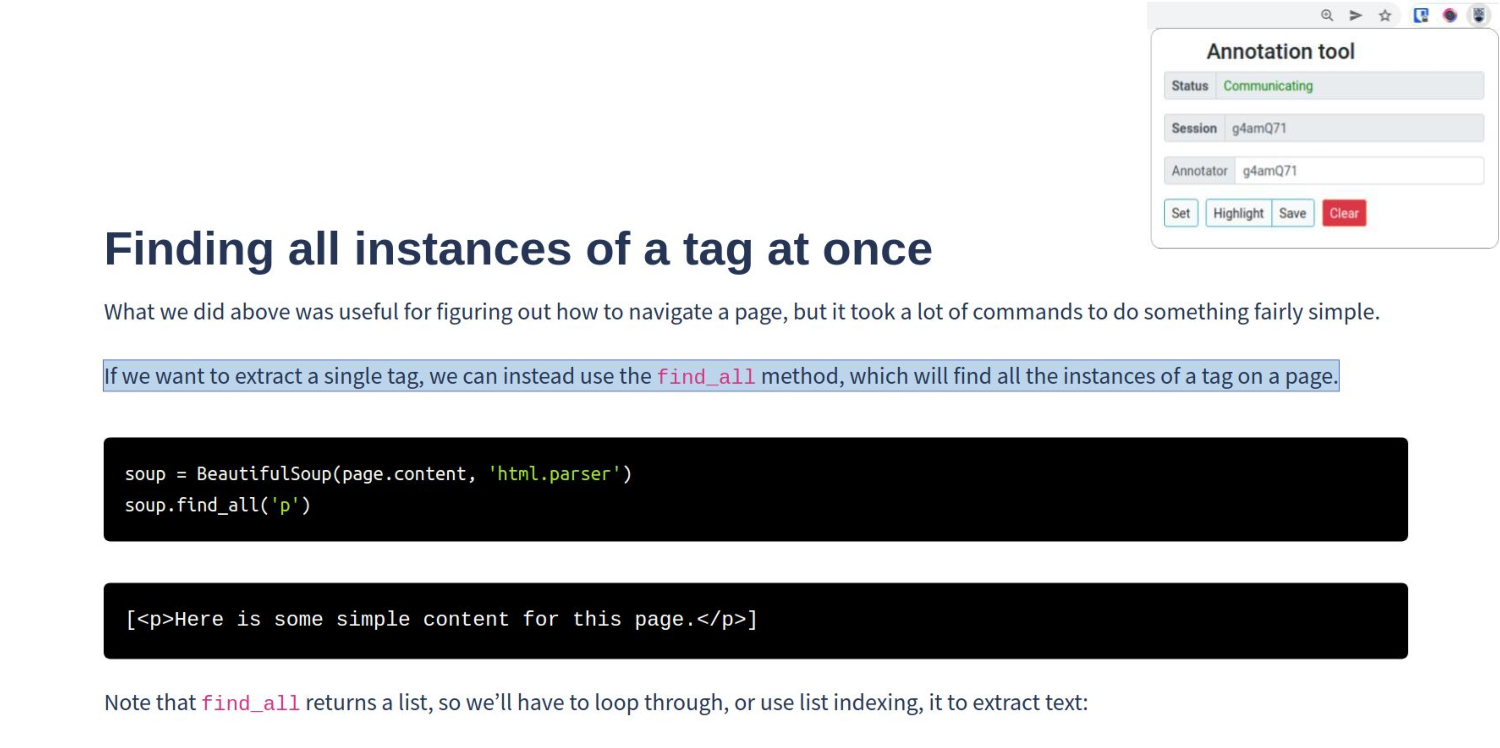
\includegraphics[width=1.0\textwidth]{cp6/manual-task.pdf}
    \caption{Study's tool context menu (top-right corner) and a sentence highlighted by a participant}
    \label{fig:artifact-pre-highlight}
\end{figure}




\subsubsection{Tool-assisted Task}
\label{cp6:procedures-tool-assisted}


In the tool-assisted task, the study tool automatically highlighted text that 
its underlying semantic-based technique identified as relevant to the participant's task.
The highlights were shown in a format similar to the one in Figure~\ref{fig:artifact-pre-highlight}, but without the need for any actions by a participant.




For this task, when a participant submitted their solution, we asked them to 
rate on a 5 points Likert scale~\cite{likert1932technique} how helpful were the highlights shown by the tool.
Figure~\ref{fig:experiment-rating} shows an example of how we gathered data about the usefulness of the text automatically identified.
Participants rated highlights on a per artifact basis.
We gather input at the artifact level because it would be too demanding for a participant 
to provide individual feedback on each of the highlights shown
in the time that we estimated and that we advertised for the study.
Section~\ref{cp6:threats} discusses  threats that arise from this decision.




\begin{figure}
\begin{mdframed}[backgroundcolor=gray!15] 
\begin{scriptsize}

\noindent \textbf{1.} Indicate whether you agree with the following statement:

\medskip

\quad \textit{The highlights in \textcolor{steelblue}{``How to extract HTTP response body from a Python requests call''} were helpful to} 

\quad \textit{correctly accomplish the task in question.}  \smallskip

\smallskip

\quad \quad \textit{(Strongly disagree)} ~$1$ - $2$ - $3$ - $4$ - $5$ ~\textit{(Strongly agree)} 


\bigskip


\noindent \textbf{2.} Indicate whether you agree with the following statement:

\medskip

\quad \textit{The highlights in \textcolor{steelblue}{``BeautifulSoup tutorial: Scraping web pages with Python''} were helpful to} 

\quad \textit{correctly accomplish the task in question.}  \smallskip

\smallskip

\quad \quad \textit{(Strongly disagree)} ~$1$ - $2$ - $3$ - $4$ - $5$ ~\textit{(Strongly agree)} 

\centering 

...

\end{scriptsize}
\end{mdframed}
\caption{Questions asking a participant to rate the usefulness of the highlights shown in two artifacts; by clicking on the name of an artifact, a participant could revisit the highlights of that artifact}
\label{fig:experiment-rating}
\end{figure}

    



\subsection{Summary of experimental procedures}


We have described experimental procedures 
where participants attempted two programming tasks each.
These procedures allowed us to gather:


\begin{enumerate}
\item a participant's submitted solution (written Python code) for each task;
\item text that participants deemed relevant in the artifacts of the control task;
\item the usefulness of the highlights shown in a tool-assisted task; and
\item any additional feedback (written text) that a participant wished to provide.
\end{enumerate}


We use this data to investigate whether 
a tool embedding a semantic-based technique helps developers complete a software task. 


\clearpage




\section{Results}
\label{cp6:results}

We organize results assessing the solutions submitted by the participants, 
comparing manual and automatically identified text as well as discussing the usefulness of the highlights shown 
by the study's tool.

\gcm{Seems like the usefulness of highlights is more important than
the comparison.}



\section{Tasks Correctness}
% \section{Does \acs{beskar} lead to more correct solutions?}
\label{cp6:correctness}



When assisted by a tool able to automatically highlight text identified as relevant to a task, we expect that a developer can produce a solution 
that is equally or more correct than the solution of a developer who attempted a task without tool support. 
To explore the correctness of the solutions submitted by participants who attempted a task 
with and without tool support, we compile their code and run it against a set of test cases 
that assess their correctness.


\subsection{Method}


The correctness of a submitted solution is measured by the number of passing test cases
when running that solution against a set of 10 test cases, specific to each task. 
A solution with compile errors has a correctness score of zero.


\smallskip
\begin{small}


\begin{equation}
    Correctness = \frac{ \text{\textit{\# of passing test cases}}}{\text{\textit{\#  of test cases}}}
\end{equation}
\end{small}

\subsection{Results}
 

\subsection{Comparison of manual and automatically identified task-relevant text}
\label{cp6:comparison}


To assist a developer to complete a task correctly, a tool that
automatically identifies text pertinent to that task would ideally 
identify text that humans have also considered as relevant.
\gcm{Why ideally? Maybe humans are terrible at identifying relevant text?}
Procedures from our control task asked participants to identify text they deemed useful. We
 compare this manually provided data against the text automatically identified.



% \paragraph{\textbf{Metrics.}}

\subsubsection{Metrics}

To investigate the overlap between the participants' manual highlights and the 
the automatic highlights identified by the study tool we use \textit{precision}, \textit{recall}~\cite{manning2010IR}, and \textit{pyramid precision}~\cite{Nenkova2004}.
We compute these metrics for each artifact of each task and report their average.


For this analysis, we follow Lotufo et al.'s procedures~\cite{Lotufo2012} and we consider any text marked by any participant as relevant.
We investigate if our tool  automatically identifies text that multiple participants deemed relevant
 via \textit{pyramid precision}. 
Details for each metric are as follows. 

\medskip

Precision measures the fraction of the text automatically identified  that participants deemed relevant (Equation~\ref{eq:precision-cp6}). 

\smallskip
\begin{small}
\begin{equation}
    Precision = \frac{
        \text{\textit{automatic highlights}~} \cap 
        \text{~\textit{manual highlights}}
    }{\text{\textit{automatic highlights}}}
\label{eq:precision-cp6}    
\end{equation}
\end{small}


Recall represents how many of all the manual highlights were identified by the semantic-based technique applied by our tool (Equation~\ref{eq:recall-cp6}). 



\smallskip
\begin{small}
\begin{equation}
    Recall = \frac{
        \text{\textit{automatic highlights}~} \cap 
        \text{~\textit{manual highlights}}
    }{\text{\textit{manual highlights}}}
\label{eq:recall-cp6}    
\end{equation}
\end{small}

\medskip


\textit{Pyramid precision} compares the text automatically identified to an optimal output, i.e., one where---for the same number of sentences---we identify sentences selected by the most number of participants (Equation~\ref{eq:pyramid-precision-cp6}). The more we identify text that more participants indicated as relevant, the higher pyramid precision is.



\smallskip
\begin{small}
\begin{equation}
    \triangle Precision = \frac{
        weight(\text{\textit{automatic highlights}~})
    }{weight(\text{\textit{optimal highlights}})}
\label{eq:pyramid-precision-cp6}    
\end{equation}
\end{small}
    


To illustrate these metrics, consider an artifact with 4 sentences $\{s_1, s_2, s_3, s_4\}$ that have been selected by $\{2, 0, 1, 1\}$ participants, respectively.
% For an output identifying two sentences for this artifact, an optimal solution would identify sentences $\{s_1, s_3\}$. 
Table~\ref{tbl:metrics-example} shows precision, pyramid precision, and recall metrics in a scenario where we output sentences $\{s_2, s_3\}$ as relevant.
    



\begin{table}[h!]
\caption{Example showing how we compute precision, recall and pyramid precision metrics}
\label{tbl:metrics-example}
\centering    
\begin{small}
\begin{threeparttable}
\rowcolors{2}{}{lightgray}
\begin{tabular}{lcc}

\textit{metric} & \textit{formula} & \textit{result} \\ 
\hline

\textit{precision} & \parbox[c][.9cm][c]{4cm}{\centering $\frac{\{s_2, s_3\}~ \cap ~\{s_1, s_3\}}{\{s_2, s_3\}} = \frac{1}{2}$} & 0.5 
\\


\textit{recall}  & \parbox[c][.9cm][c]{4cm}{\centering $\frac{\{s_2, s_3\}~ \cap ~\{s_1, s_3\}}{\{s_1, s_3,  s_4\}} = \frac{1}{3}$}  & 0.33 
\\

$\triangle$ \textit{precision}  & \parbox[c][.9cm][c]{4cm}{\centering $\frac{weight(s_2) + weight(s_3)}{weight(optimal)} = \frac{0 + 1}{3} $}  & 0.33 
\\

\end{tabular}
\end{threeparttable}
\end{small}
\end{table}



% \smallskip
% \begin{small}
% \begin{equation}
% \begin{split}
% \triangle  Precision(s_2, s_3) = ( 0 + 1) \div 3 =  0.33 \\
% \triangle  Precision(s_1, s_2) = ( 2 + 0) \div 3 =  0.66 \\
% \triangle  Precision(s_1, s_3) =  ( 2 + 1) \div 3 =  1.00 \\
% \label{eq:pyramid-precision-cp6} 
% \end{split}   
% \end{equation}
% \end{small}



% Note that pyramid precision is equal or lower than precision. For example, $Precision(s_1, s_3) = Precision(s_3, s_4) = 1.0$, but 
% results for pyramid precision differ, i.e., 
% $\triangle Precision(s_1, s_3) = 1.0$ and $\triangle Precision(s_3, s_4) = 0.66$. This allows us to check if our tool 
% identified the text deemed relevant by most of the participants who inspected an artifact.



% \paragraph{\textbf{Data.}}
\subsubsection{Data}

Participants who indicated what text was relevant to their assigned control task produced a total of 415 highlights with an average of 7 highlights (std $\pm 3$) per artifact inspected.
On average, this comprises 9\% of the entire content of the artifacts in our experiment. 


Some participants also selected code snippets as relevant to a task---a threat that we discuss in Section~\ref{cp6:threats}. 
Code snippets account for 30\% of the highlights produced, but we remove them from our analysis since our semantic-based approach 
operates on text only. For the textual highlights,
Krippendorf's alpha indicates good agreement of what text in an artifact participants deemed relevant ($\alpha = 0.68$)~\cite{Krippendorff1980, passonneau2006}.
We compare these manually produced highlights to the text automatically identified by our tool.



% \subsubsection{Results}


% \paragraph{\textbf{Results.}}
\subsubsection{Results}



Table~\ref{tbl:comparison-task-wise} summarizes the average of precision, pyramid precision, and recall metrics for each of the tasks in the experiment.
Precision scores range from 0.55 to 0.68, while pyramid precision scores range from 0.55 to 0.57, which suggests that our tool failed to identify some of the text that participants deemed the most relevant.



The results in Table~\ref{tbl:comparison-task-wise} corroborate 
the correctness scores detailed in Figure~\ref{fig:correctness-by-task}. For example, 
in the \texttt{distances} task, participants who performed the task with tool support had solutions less correct than participants in the control group.
This was the task with the lowest precision, recall and pyramid precision values. 
In contrast, the task where participants assisted by our tool obtained the best correctness scores, namely \texttt{titanic}, is the one with the best precision, recall and pyramid precision values.





\begin{table}
\caption{Evaluation metrics per artifact type}
\label{tbl:comparison-overall}
\centering    
% \begin{scriptsize}
\begin{threeparttable}
\begin{tabular}{lcc}

  & \textbf{precision} & \textbf{recall}  \\ 
\hline

Distances & 0. & 0.
\\

NYTimes  & 0. & 0. 
\\

Titanic & 0. & 0.
\\

\hline


\textbf{overall} & 0. & 0.
\\

\hline

\end{tabular}
\end{threeparttable}
% \end{scriptsize}
\end{table}




Table~\ref{tbl:comparison-artifact-type-wise} details evaluation metrics artifact-type wise. 
Stack Overflow posts and API documentation have the highest precision scores. For these types of artifacts, pyramid precision indicates that the 
text automatically identified on Stack Overflow was the text that several participants deemed relevant. 
The same does not apply to API documentation, i.e., our tool failed to detect a portion of the text that many participants deemed relevant. 
Miscellaneous web pages were the artifact type with the lowest scores. As we detail in Section~\ref{cp6:usefulness},
participants indicated that the text identified for this type of artifact was the least useful.



\begin{table}
\caption{Evaluation metrics per task type}
\label{tbl:comparison-artifact-type-wise}
\centering    
% \begin{scriptsize}
\begin{threeparttable}
\rowcolors{2}{}{lightgray}
\begin{tabular}{lccc}




& \textbf{precision} & $\triangle$ \textbf{precision} & \textbf{recall} \\ 
\hline

API documentation & 0.65 & 0.55 & 0.59
\\

Stack Overflow posts  & 0.66 & 0.62 & 0.63
\\

Miscellaneous web pages & 0.53 & 0.53 & 0.54
\\


\hline
\end{tabular}
\end{threeparttable}
% \end{scriptsize}
\end{table}



\gcm{And how does this compare to Chapter 5 results?}

\art{add comparison. }






% \section{Is \acs{beskar} useful?}
\section{Result: Usefulness Analysis}
\label{cp6:usefulness}




% caused by individual differences between the participants who performed a task with and without tool support, what can justify a similar level of correctness in the results; or the presence (or lack) of overlap between the manual and automatically identified 
% text. 
% However, this does not imply that the tool helped participants accomplish their task. 


To further explore if the highlights shown by the tool were helpful, we also asked a participant 
to indicate whether the highlights assisted them complete their assigned task. 
In this section, we described results for this analysis. 



\subsection{Method}



\subsection{Results}



% We use a diverging stacked bar chart~\cite{Heiberger2014} to analyze the  Likert scale
% responses on the usefulness of the text automatically identified.


% Usefulness indicates the percentage of responses agreeing or disagreeing with whether sentences
% automatically highlighted assisted a participant in completing a task.


% \smallskip
% \begin{small}

% \begin{equation}
% Usefulness = \frac{
%     \text{\textit{\# of responses at i}}
% }{
%     \text{\textit{total \# of responses}}
% }
% \end{equation}
        

% \begin{equation*}
% i \in \{ 
%     \text{\textit{
%         (strongly) agree, neither agree or disagree, (strongly) disagree
%     }}  
% \}
% \end{equation*}
% \end{small}





% \subsubsection{Written Feedback}

 
% We use qualitative methods to analyze participants' responses to the open-ended questions. 

% \art{Think this through...}



\subsection{Summary of results}


Results from our experiment suggest that
participants find the text automatically identified
most useful when the semantic based technique applied by our tool 
identifies text that humans deemed relevant to a task.
In such scenario, we observe that participants 
produced more correct solutions. 
However, when it failed to detect the text deemed relevant,
participants found the tool's output not as useful and 
their solutions had more errors. 
These results suggests that our tool might positively or negatively 
impact how a developer completes a task. 



\subsection{Threats to Validity}
\label{cp6:threats}




Our experiment compares solutions submitted by participants who attempted each task with and without tool support. 
This represents a between groups design~\cite{Lazar2017-cp3} and we discuss threats inherent to it. 



Since we compare results from different participants, our analysis might be subject to substantial 
impact from individual differences~\cite{Lazar2017-cp3}. 
For example, participants who performed a task with tool support may have been more experienced than participants 
who did the same task without tool support what affects correctness scores.
As another example,  participants' skill and background 
influences the text that they indicate as relevant in the control task as well 
what text they perceive as useful in the tool-assisted task. 
We minimized these threats by recruiting participants of varied background and randomly
assigning tasks to each participant.



The tasks in our experiment impact generalizability. 
Although we opted for simple tasks, we ensured they 
modules used in our tasks were representative. 
For example, we found open-source systems\footnote{\url{https://github.com/ArchiveBox/ArchiveBox/issues/18}} using \texttt{BeautifulSoup} 
with function calls similar to the ones needed to complete the \texttt{NYTimes} task.
Nonetheless, there are clear differences in the artifacts one can gather 
based on the domain or programming language of a task~\cite{baltes2020}.
Hence, we consider other domains and a wider range of task 
and artifacts for future work. 



The selection of tasks also affects our conclusions. We opted for Python programming tasks that 
required writing code, which we use to assess correctness. 
As observed by other researchers~\cite{satterfield2020, meyer2020}, developers
work on many different tasks, some of which focus on code~\cite{Meyer2017}
while others on information seeking~\cite{gonccalves2011}, e.g., finding duplicated bug reports or researching visualization libraries to identify the most suitable one~\cite{satterfield2020}.
Had we decided to use information-seeking tasks, participants could have produced a different set of highlights,
perhaps selecting fewer code snippets. 
Given that 
our experiment was completely remote, instructing participants on how to perform information-seeking 
tasks would have been more difficult. Furthermore, objectively judging their correctness 
would also be more strenuous, which would lead to a different experiment with challenges and risks of its own.




The fact that we consider the text marked by any participant as relevant 
also affect our conclusions. 
We refrain from excluding text selected by a few participants from our analysis 
for reasons similar to the ones in our characterization of task-relevant information (Chapter~\ref{ch:characterizing}). That is, the text marked by these participants may still contain valuable information. 
We minimize this threat by reporting both precision and pyramid precision, where we observe that 
our approach failed to detect the text that multiple participants deemed relevant
for some tasks or types of artifacts. 



Concerning the text automatically identified by our tool, we gather usefulness at the artifact level.
Suppose we had gathered usefulness at the sentence level. In that case, we could have used this information 
to further refine our analysis, for example, reporting precision and recall 
at different usefulness levels or computing accuracy based on the participants' input, as done by Xu et al~\cite{Xu2017}. 
However, asking participants to provide feedback at the sentence level would have considerably increased the time we estimated that the experiment would take,
which would impact recruitment. We weighed the benefits and drawbacks of a fine-grained or more coarse-grained 
analysis, and we opted for the latter so that this would not be a barrier to people deciding on 
whether to participate in our experiment.
\section{Summary}
\label{cp6:summary}


% \art{ask about summary and better way to position conclusions from the experiment}

In this chapter, we presented an experiment to evaluate whether \acs{tool},
 a tool that embeds a semantic-based technique, assists a developer working on a software task. 
The experiment examined how 24 participants with software development backgrounds attempted 
two programming tasks with or without such a tool. 
Results from this experiment indicate that, 
participants found the text automatically identified and shown by our tool useful in two 
out of the three types of artifacts that assisted them completing their assigned tasks,
where our automatic approach identified on average 58\% of the text that participants deemed relevant. 
These results encourage further exploration of semantic-based techniques, 
embedding them into tools that ultimately facilitate a developer's work.




% \gcm{Sorry if I missed it but do you outline the number of artifacts and type of artifacts per task?}
% \art{sorry. I will add that to the Artifacts session}



% \art{I'm trying to set results in a manner similar to how we did in the  (``Task-Relevant Knowledge Identification'')ICPC paper---present an overview of what we evaluate in the section, describe the method of evaluation and then, the results.}


% \section{Summary}
\label{cp6:summary}


% \art{ask about summary and better way to position conclusions from the experiment}

In this chapter, we presented an experiment to evaluate whether \acs{tool},
 a tool that embeds a semantic-based technique, assists a developer working on a software task. 
The experiment examined how 24 participants with software development backgrounds attempted 
two programming tasks with or without such a tool. 
Results from this experiment indicate that, 
participants found the text automatically identified and shown by our tool useful in two 
out of the three types of artifacts that assisted them completing their assigned tasks,
where our automatic approach identified on average 58\% of the text that participants deemed relevant. 
These results encourage further exploration of semantic-based techniques, 
embedding them into tools that ultimately facilitate a developer's work.

%  (``Task-Relevant Knowledge Identification'')